\input{../../../.preambles/02-lab_work}
\newgeometry{top=1.5cm, bottom=1.5cm, left=1cm, right=1cm}
\begin{document}
    \begin{table}[h!]
        \center
        \begin{tabular}{|C{.5}|C{.2}|C{.25}|}
            \hline
            \multicolumn{1}{|c|}{\multirow{4}{*}{Лабораторная работа № 3}} &
            Студент, группа & {{ student }}, Ф-369 \\ \cline{2-3}
            & Дата выполнения & 19.04.2013 \\ \cline{2-3}
            & Подпись &  \\ \cline{2-3}
            Память 4x1 & Дата отчёта & \\ \cline{2-3}
            & Оценка &  \\ \cline{2-3}
            & Подпись &  \\ \hline
        \end{tabular}
    \end{table}

    \emph{Цель работы:} научиться работать со сложными элементами на примере
    RS-триггеров и составить схему памяти 4x1 в программной среде
    \emph{Quartus}.

    Схема памяти и ее временная диаграмма \(\bigl(\)адрес элементарной ячейки
    памяти \( A \) изменяется последовательно от 0 до 3, происходит смена
    уровня сигнала записи и чтения \emph{R/nW}, на вход \emph{data\_IN} данные
    для записи подаются случайным образом, вход \( C \) -- синхросигнал, выходы
    \( Q_{00\ldots11} \) -- состояния соответствующих элементарных ячеек, выход
    \emph{data\_OUT} -- считанные данные\(\bigr)\) представлены на рисунке
    \ref{pic_memory}.
    
    \begin{figure}[h!]
        \center
        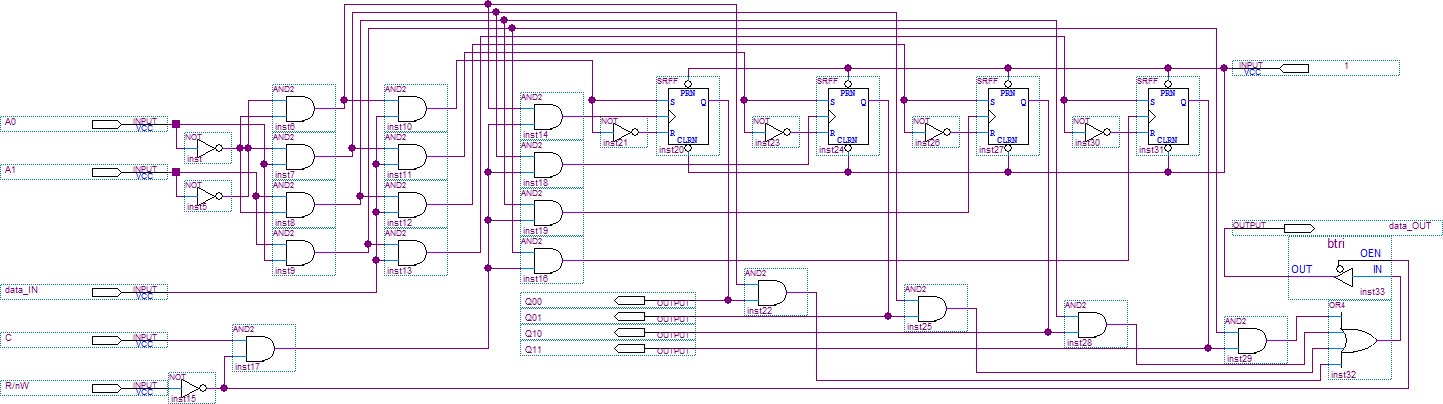
\includegraphics[width=1\textwidth]{sram} \vspace*{2em}\\
        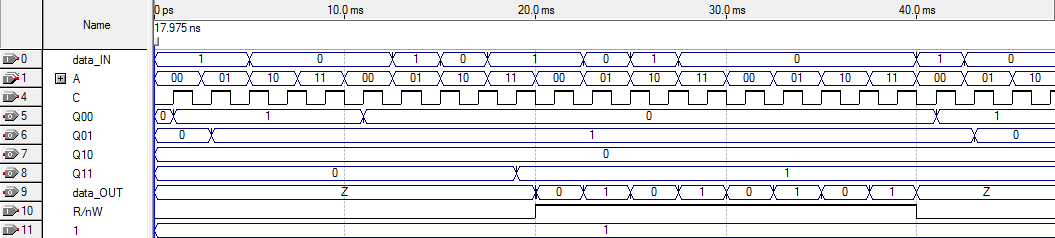
\includegraphics[width=.9\textwidth]{sram_time}
        \caption{Схема памяти и ее временная диаграмма}
        \label{pic_memory}
    \end{figure}    
\end{document}
